\documentclass[a4paper]{article}

% --- Packages ---

\usepackage{a4wide}
\usepackage[utf8]{inputenc}
\usepackage{amsmath}
\usepackage{mathtools}
\usepackage{amssymb}
\usepackage[english]{babel}
\usepackage{mdframed}
\usepackage{systeme,}
\usepackage{lipsum}
\usepackage{relsize}
\usepackage{caption}
\usepackage{tikz}
\usepackage{tikz-3dplot}
\usetikzlibrary{shapes.geometric}
\usepackage{pgfplots}
\usepackage{pgfplotstable}
\pgfplotsset{compat=newest}%1.7}
\usepackage{harpoon}%
\usepackage{graphicx}
\usepackage{wrapfig}
\usepackage{subcaption}
\usepackage{authblk}
\usepackage{float}
\usepackage{listings}
\usepackage{xcolor}
\usepackage{chngcntr}
\usepackage{amsthm}
\usepackage{comment}
\usepackage{commath}
\usepackage{hyperref}%Might remove, adds link to each reference
\usepackage{url}
\usepackage{calligra}
\usepackage{pgf}

% --- Bibtex ---
% To run our bibliography, we need to compile the ref document
% `biber main` or `biber ref` in the terminal
% We can compile the document with `pdflatex main` or `latex main`

\usepackage{csquotes}
\usepackage[
    %backend=biber,
    backend = biber,
    style=phys,
    sorting=ynt,
]{biblatex}

%\addbibresource{ref.bib}


% --- Commands --- 

\newcommand{\w}{\omega}
\newcommand{\trace}{\text{Tr}}
\newcommand{\grad}{\mathbf{\nabla}}
%\newcommand{\crr}{\mathfrak{r}}
\newcommand{\laplace}{\nabla^2}
\newcommand{\newparagraph}{\vspace{.5cm}\noindent}

% --- Math character commands ---

\newcommand{\curl}[1]{\mathbf{\nabla}\times \mathbf{#1}}
\newcommand{\dive}[1]{\mathbf{\nabla}\cdot \mathbf{#1}}
\newcommand{\res}[2]{\text{Res}(#1,#2)}
\newcommand{\fpartial}[2]{\frac{\partial #1}{\partial #2}}
\newcommand{\rot}[3]{\begin{vmatrix}\hat{x}&\hat{y}&\hat{z}\\\partial_x&\partial_y&\partial_z\\#1&#2&#3 \end{vmatrix}}
\newcommand{\average}[1]{\langle #1 \rangle}
\newcommand{\ket}[1]{|#1\rangle}
\newcommand{\bra}[1]{\langle #1|}


%  --- Special character commands ---

\DeclareMathAlphabet{\mathcalligra}{T1}{calligra}{m}{n}
\DeclareFontShape{T1}{calligra}{m}{n}{<->s*[2.2]callig15}{}
\newcommand{\crr}{\mathcalligra{r}\,}
\newcommand{\boldscriptr}{\pmb{\mathcalligra{r}}\,}


\title{Solving the time independent Schrödinger equatio}
\author{Author : Andreas Evensen}
\date{Date: \today}

% --- Code ---

\definecolor{codegreen}{rgb}{0,0.6,0}
\definecolor{codegray}{rgb}{0.5,0.5,0.5}
\definecolor{codepurple}{rgb}{0.58,0,0.82}
\definecolor{backcolour}{rgb}{0.95,0.95,0.92}

\lstdefinestyle{mystyle}{
    backgroundcolor=\color{backcolour},   
    commentstyle=\color{codegreen},
    keywordstyle=\color{magenta},
    numberstyle=\tiny\color{codegray},
    stringstyle=\color{codepurple},
    basicstyle=\ttfamily\footnotesize,
    breakatwhitespace=false,         
    breaklines=true,                 
    captionpos=b,                    
    keepspaces=true,                 
    numbers=left,                    
    numbersep=5pt,                  
    showspaces=false,                
    showstringspaces=false,
    showtabs=false,                  
    tabsize=2
}

\lstset{style=mystyle}

\begin{document}

\begin{titlepage}
    \begin{center}
        \vspace*{1cm}
        
        \Huge
        \textbf{Solving the time independent Schrödinger equation}
        
        \vspace{0.5cm}
        \LARGE
        FK8029 - Computational Physics
        
        \vspace{1.5cm}
        
        \textbf{Andreas Evensen}
        
        \vfill
        
        %\includegraphics[width=0.4\textwidth]{UiO_Segl_pantone.eps}
        
        \Large
        Department of Physics\\
        Stockholm University\\
        Sweden\\
        \today
    \end{center}
\end{titlepage}

%\maketitle

%\printbibliography
\tableofcontents

\section{Introduction}
How does a quantum mechanical system behave?
What does the wave-function look like? And how does it change depending on the energy of the system?
In quantum mechanics, the Schrödinger equation is used to describe the behavior of a system.
It allows us to calculate the wave-functions of a system and their corresponding energies.
However, this equation is not always easy to solve. Therefore, we often need to use numerical methods to solve it.

\newparagraph
In this report, we will solve the known Schrödinger equation for a one-dimensional system with the potential of a harmonic oscillator.
This will be achieved by using two numerical methods, matrix diagonalization and the inverse power iteration method.
We will compare the two methods against each-other, and we will also try other potentials to see how the wave-function changes.

\newpage
\section{Theory \& Method}
Schrödinger's time-independent equation is a second order differential equation that describes the behavior of a quantum mechanical system.
It's given by the following expression:
\begin{align}
    \hat{H}\ket{\psi} &= E\ket{\psi},\label{eq: schrödinger}\\
    \hat{H} &= -\frac{\hbar^2}{2m}\laplace + V(x),\nonumber
\end{align}where $V(x)$ is the potential describing the system. The potential of a harmonic oscillator is given by $V(x) = \frac{1}{2}m\w^2x^2$,
which allows for rewriting the Hamiltonian in a dimensionless form:
\begin{align*}
    \hat{H} = -\frac{1}{2}\laplace + \frac{1}{2}z^2.
\end{align*}The potential is shown in the figure below, \ref{fig: harmonic oscillator potential}, where the energy is plotted against the position.

\begin{figure}[H]
    \centering
    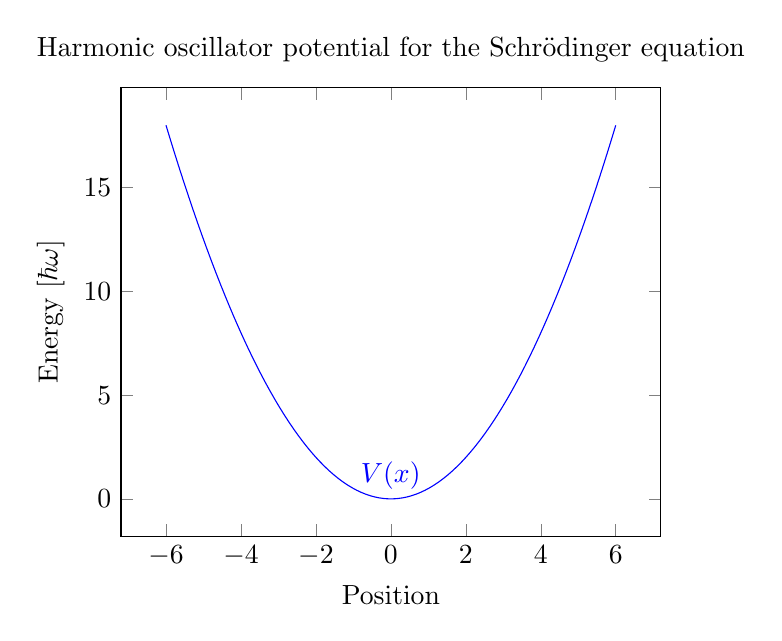
\begin{tikzpicture}
        \begin{axis}[
                xlabel = {Position},
                ylabel = {Energy [$\hbar\w$]},
                title = {Harmonic oscillator potential for the Schrödinger equation},
                legend pos = north west,
                domain = -6:6,
                samples = 100,
            ]
            \addplot[thin, blue] {x * x / 2} node[pos = 0.5, above] {$V(x)$};
        \end{axis}
    \end{tikzpicture}
    \caption{Potential of a harmonic oscillator.}
    \label{fig: harmonic oscillator potential}
\end{figure}\noindent
In order to solve the eigen-equation above, \eqref{eq: schrödinger}, we will use two numerical methods, matrix diagonalization and the inverse power iteration method.
The matrix diagonalization method is a direct method what involves solving the equation $\det(\hat{H}) = 0$, i.e. finding the eigenvalues of the Hamiltonian, and their corresponding eigenvectors.
For this, we discretize the space and use a finite difference method to obtain the Hamiltonian matrix; both the three-point and five-point stencil will be used. 
\begin{align}
    \frac{d^2 f_i}{dz^2} &= \frac{f_{i+1} - 2f_i + f_{i-1}}{dz^2} + \mathcal{O}(dz^2),\label{eq: 3p stencil}\\
    \frac{d^2 f_i}{dz^2} &= \frac{-f_{i + 2} + 16f_{i+1} - 30f_i + 16f_{i-1} - f_{i - 2}}{12dz^2} + \mathcal{O}(dz^4).\label{eq: 5p stencil}
\end{align}The other method, inverse power iteration, is an iterative method that allows us to find the eigenvalues of the Hamiltonian.
This allows us to find the eigenvalues of the Hamiltonian, and their corresponding eigenvectors, given an approximate value of the eigenvalue. The matrix still has to be constructed, but for the sake of this report, only the five-point stencil, eq \eqref{eq: 5p stencil} was used.
Inverse power method is described by the following equations:
\begin{align}
    \lim_{i\to\infty}&\frac{\mathbf{v_i}^\dagger (\hat{H - Is})^{-1}\mathbf{v_i}}{\mathbf{v}^\dagger\mathbf{v}} = \frac{1}{\lambda - s},\label{eq: inverse power iteration1}\\
    \mathbf{v}_{i + 1} &= (\hat{H - I\cdot s})^{-1}\mathbf{v}_i,\label{eq: inverse power iteration2}
\end{align}where $s$ is the shift applied to the Hamiltonian, in order to converge to the desired eigenvalue.
Thus, in order to effectively use this an approximated eigenvalue is needed, which can be found by using the direct diagonalization method with lower resolution than the desired result.
It's however important to note, the smaller the discretization of the Hamiltonian, the more accurate the result will be for the diagonalization method for larger eigenvalues.
This however also implies that for increasing number of eigen-states included, the direct method will be more accurate for the lower eigenstates, and the inverse power iteration method will be more accurate for the higher eigenstates;
with the good guesses for the shift applied.

\newparagraph
Due to the nature of this system, we also include that the ladder operators, $\hat{a}$ and $\hat{a}^\dagger$, can be used to find the eigen-states of the system, and their corresponding energies, by performing the matrix operator multiplication described in eq \eqref{eq: schrödinger}.
The ladder operators, are defined by:
\begin{align*}
    \hat{a} &= \sqrt{\frac{m\w}{2\hbar}}\left(\hat{x} + \frac{i}{m\w}\hat{p}\right),\\
    \hat{a}^\dagger &= \sqrt{\frac{m\w}{2\hbar}}\left(\hat{x} - \frac{i}{m\w}\hat{p}\right),
\end{align*}and with the change of basis to the dimensionless form, we get:
\begin{align}
    \hat{a} &= \frac{1}{\sqrt{2}}\left(z + \frac{d}{dz}\right),\label{eq: down}\\
    \hat{a}^\dagger &= \frac{1}{\sqrt{2}}\left(z - \frac{d}{dz}\right)\label{eq: up}.
\end{align}This then allows us to find the eigen-state $i$ by applying the creation operator on the previous state, i.e.
\begin{align*}
    \ket{\psi_{i + 1}} = \hat{a}^\dagger\ket{\psi_i}.
\end{align*}This is done until the desired number of eigen-states are found. The operators are then described in matrix form of the following, in the basis of the harmonic oscillator:
\begin{align*}
    \hat{a}^\dagger &= \begin{pmatrix}
        0 & 0 & 0 & 0 & \dots & 0 & \dots \\
        \sqrt{1} & 0 & 0 & 0 & \dots & 0 & \dots \\
        0 & \sqrt{2} & 0 & 0 & \dots & 0 & \dots \\
        0 & 0 & \sqrt{3} & 0 & \dots & 0 & \dots \\
        \vdots & \vdots & \vdots & \ddots & \ddots & \dots & \dots \\
        0 & 0 & 0 & \dots & \sqrt{n} & 0 & \dots & \\
        \vdots & \vdots & \vdots & \vdots & \vdots & \ddots & \ddots
    \end{pmatrix},\\
    \hat{a} &= \begin{pmatrix}
    0 & \sqrt{1} & 0 & 0 & \dots & 0 & \dots \\
    0 & 0 & \sqrt{2} & 0 & \dots & 0 & \dots \\
    0 & 0 & 0 & \sqrt{3} & \dots & 0 & \dots \\
    0 & 0 & 0 & 0 & \ddots & \vdots & \dots \\
    \vdots & \vdots & \vdots & \vdots & \ddots & \sqrt{n} & \dots \\
    0 & 0 & 0 & 0 & \dots & 0 & \ddots \\
    \vdots & \vdots & \vdots & \vdots & \vdots & \vdots & \ddots
    \end{pmatrix}.
\end{align*}Both these matrices are $n\times n$ matrices, where $n$ is the number of eigen-states desired.

\section{Result \& Discussion}
In this section we solve the above theory using a discretization of the spacial domain $z_{min}= -6$ and $z_{max} = 6$, with $n - 2$ number of interior points. 
Each section describes a specific potential function $V(z)$, in our dimensionless basis.

\subsection{Harmonic Oscillator}
In this section the potential $V(z) = \frac{1}{2}z^2$ is used, and all results below are given by this potential unless otherwise specified.
The eigen-states of a harmonic oscillator are well known, and there exists an analytical solution to the problem, namely that the energy corresponding to the eigen-state is given by:
\begin{align*}
    E_n = \left(n + \frac{1}{2}\right)\hbar\w.
\end{align*}We will use this to compare the results of our numerical methods. Firstly, we look at the probability distribution $\abs{\psi_i}^2$ of the wave-functions, for the direct diagonalization method.
Since the eigen-states are well known, we can directly compare the visual results of the wave-function to the analytical solution.
\begin{figure}[H]
    \centering
    \begin{subfigure}{0.45\textwidth}    
        \begin{tikzpicture}[scale = 0.75]
            \begin{axis}[
                xlabel = {Position},
                ylabel = {$\abs{\psi}^2$},
                grid = both,
                grid style={line width=.1pt, draw=gray!10},
                major grid style={line width=.2pt,draw=gray!50},
                minor tick num=2,
                title = {Probability distribution $\abs{\psi_i}^2$},
                legend pos = south east,
            ]
            \addplot[thin, blue] table [x index = 0, y index = 1, header = true] {code/5pt.dat};
            \addlegendentry{$\psi_0$}
            \addplot[thin, red] table [x index = 0, y index = 3, header = true] {code/5pt.dat};
            \addlegendentry{$\psi_2$}
            \end{axis}
        \end{tikzpicture}
        \caption{Probability distribution for even wave-functions.}
        \label{fig: even wave-functions, dm}
    \end{subfigure}
    \hfill
    \begin{subfigure}{0.45\textwidth}    
        \begin{tikzpicture}[scale = 0.75]
            \begin{axis}[
                xlabel = {Position},
                ylabel = {$\abs{\psi}^2$},
                grid = both,
                grid style={line width=.1pt, draw=gray!10},
                major grid style={line width=.2pt,draw=gray!50},
                minor tick num=2,
                title = {Probability distribution $\abs{\psi_i}^2$ },
                legend pos = south east,
            ]

            \addplot[thin, blue] table [x index = 0, y index = 2, header = true] {code/5pt.dat};
            \addlegendentry{$\psi_1$}
            \addplot[thin, red] table [x index = 0, y index = 4, header = true] {code/5pt.dat};
            \addlegendentry{$\psi_3$}
            \end{axis}
        \end{tikzpicture}
        \caption{Probability distribution for odd wave-functions.}
        \label{fig: odd wave-functions, dm}
    \end{subfigure}
    \caption{Probability distribution of the wave-functions using direct diagonalization}
    \label{fig: five point stencil}
\end{figure}\noindent
The solutions of the probability distribution of the wave-function is as expected, where one observes a peak at the centroid of the potential well for the ground-state.
The distribution the follows the shape of the potential well, and the higher the energy of the eigen-state, the more nodes the wave-function will have, which is also expected.

\newparagraph
The direct diagonalization is then compared with the two methods to obtain the matrix representation of the Hamiltonian, the three-point and five-point stencil.
Since the three-point stencil has a lower resolution, it's expected that the error of the eigenvalues will be larger than the five-point stencil, i.e. the $\mathcal{O}(dz^2)$ versus $\mathcal{O}(dz^4)$ term.
We find that the three-point stencil indeed performs worse than the five-point stencil for the first eigen-states, where we have computed the difference between the analytical solution and the numerical solution of the eigen-value.
However, after the first few eigen-states, the three-point and five-point stencil performs in comparison to each other, as seen in figure \ref{fig: accucary, dm}.

\newparagraph
Since the five-point stencil performs better for the first eigen-states, we compare the eigen-value of the five-point stencil to that of the analytical solution.
From figure \ref{fig: dm, eigenvalue comparison} it's seen that the numerical solution is in good agreement for the first $30$--$40$ eigen-states, where the solutions overlap.
The difference in the eigen-values is then increasing after this point, and the numerical solution deviates from the analytical solution.
To further improve upon this, we could either increase the resolution of the Hamiltonian matrix, or implement seven point stencil, which would increase the accuracy of the eigen-values for the numerical solution.

\begin{figure}[H]
    \centering
    \begin{subfigure}{0.45\textwidth}    
        \begin{tikzpicture}[scale = 0.75]
            \begin{loglogaxis}[
                xlabel = {Eigen-state},
                ylabel = {$\abs{\Delta E}$},
                grid = both,
                grid style={line width=.1pt, draw=gray!10},
                major grid style={line width=.2pt,draw=gray!50},
                minor tick num=2,
                title = {Accuarcy of two methods},
                legend pos = south east,
            ]
            \addplot[thin, blue] table [x index = 0, y index = 1, header = true] {code/compare.dat};
            \addlegendentry{$\hat{H}_{3}$};
            \addplot[thin, red] table [x index = 0, y index = 2, header = true] {code/compare.dat};
            \addlegendentry{$\hat{H}_{5}$};
            \end{loglogaxis}
        \end{tikzpicture}
        \caption{Accuracy the three point-,\\ and five point stencil.}
        \label{fig: accucary, dm}
    \end{subfigure}
    \hfill
    \begin{subfigure}{0.45\textwidth}    
        \begin{tikzpicture}[scale = 0.75]
            \begin{loglogaxis}[
                xlabel = {Eigen-state},
                ylabel = {$E$},
                grid = both,
                grid style={line width=.1pt, draw=gray!10},
                major grid style={line width=.2pt,draw=gray!50},
                minor tick num=2,
                title = {Eigen value comparison },
                legend pos = south east,
            ]

            \addplot[thin, blue] table [x index = 0, y index = 1, header = true] {code/exact.dat};
            \addlegendentry{$E_{\text{exact}}$};
            \addplot[thin, red] table [x index = 0, y index = 2, header = true] {code/exact.dat};
            \addlegendentry{$E_{\text{numerical}}$};
           \end{loglogaxis}
        \end{tikzpicture}
        \caption{Comparison of eigenvalues for the 5 point stencil and the exact solution}
        \label{fig: dm, eigenvalue comparison}
    \end{subfigure}
    \caption{Comparison of the direct diagonalization method.}
    \label{fig: comparison}
\end{figure}\noindent
In order to validate our results further, we also implement the inverse power iteration method to find the eigen-states of the system, using eq \eqref{eq: inverse power iteration1} -- \eqref{eq: inverse power iteration2}.
The results of the probability distribution of the wave-functions are shown in figure \ref{fig: inverse power iteration} and are in good agreement with the direct diagonalization method.
Since this method does not require the Hamiltonian matrix to be diagonalized, it's a faster method to find a specific eigen-state of the system, given a good guess for the shift $s$. Below, in figure \ref{fig: inverse power iteration}, the probability distribution for a few eigen-states are shown.
Since this method is not suited for finding all the eigen-values, no meaningful comparison between the two numerical methods can be obtained, however the difference between the analytical solution and the iterative method is show below in figure \ref{fig: inverse comparison}.
\begin{figure}[H]
    \centering
    \begin{tikzpicture}[scale = 0.7]
        \begin{axis}[
                xlabel = {Eigen-state},
                ylabel = {$\abs{\Delta E}$},
                title = {Comparison of eigenvalues},
                grid = both,
                grid style={line width=.1pt, draw=gray!10},
                major grid style={line width=.2pt,draw=gray!50},
                minor tick num=2,
            ]
           \addplot[thin, blue] table[x index = 0, y index = 1, header = true] {code/compare_inverse.dat};
        \end{axis}
    \end{tikzpicture}
    \caption{Comparison of the eigenvalues for the inverse power iteration method.}
    \label{fig: inverse comparison}
\end{figure}\noindent
As seen in the above figure, the difference between the numerical and analytical solution is less than with the direct diagonalization method.

\begin{figure}[H]
    \centering
    \begin{subfigure}{0.45\textwidth}    
        \begin{tikzpicture}[scale = 0.75]
            \begin{axis}[
                xlabel = {Position},
                ylabel = {$\abs{\psi}^2$},
                grid = both,
                grid style={line width=.1pt, draw=gray!10},
                major grid style={line width=.2pt,draw=gray!50},
                minor tick num=2,
                title = {Probability distribution $\abs{\psi_i}^2$},
                legend pos = south east,
            ]
            \addplot[thin, blue] table [x index = 0, y index = 1, header = true] {code/inverse.dat};
            \addlegendentry{$\psi_0$}
            \addplot[thin, red] table [x index = 0, y index = 3, header = true] {code/inverse.dat};
            \addlegendentry{$\psi_2$}
            \end{axis}
        \end{tikzpicture}
        \caption{Probability distribution for even wave-functions.}
        \label{fig: even wave-functions, ipi}
    \end{subfigure}
    \hfill
    \begin{subfigure}{0.45\textwidth}    
        \begin{tikzpicture}[scale = 0.75]
            \begin{axis}[
                xlabel = {Position},
                ylabel = {$\abs{\psi}^2$},
                grid = both,
                grid style={line width=.1pt, draw=gray!10},
                major grid style={line width=.2pt,draw=gray!50},
                minor tick num=2,
                title = {Probability distribution $\abs{\psi_i}^2$},
                legend pos = south east,
            ]
            \addplot[thin, blue] table [x index = 0, y index = 2, header = true] {code/inverse.dat};
            \addlegendentry{$\psi_1$}
            \addplot[thin, red] table [x index = 0, y index = 4, header = true] {code/inverse.dat};
            \addlegendentry{$\psi_3$}
            \end{axis}
        \end{tikzpicture}
        \caption{Probability distribution for odd wave-functions.}
        \label{fig: odd wave-functions, ipi}
    \end{subfigure}
    \caption{Probability distribution of the wave-functions for the harmonic oscillator using inverse power iteration.}
    \label{fig: inverse power iteration}
\end{figure}

\subsection{Another potential}
If we instead have the following potential $V(z) = 0.5\left(z^2 + \exp\left[-\abs{z}\right]\right)$, there exists no known analytical solution to the problem.
We thus have to rely on the numerical methods to find the eigen-states of the system.


\begin{figure}[H]
    \centering
    \begin{subfigure}{0.45\textwidth}
        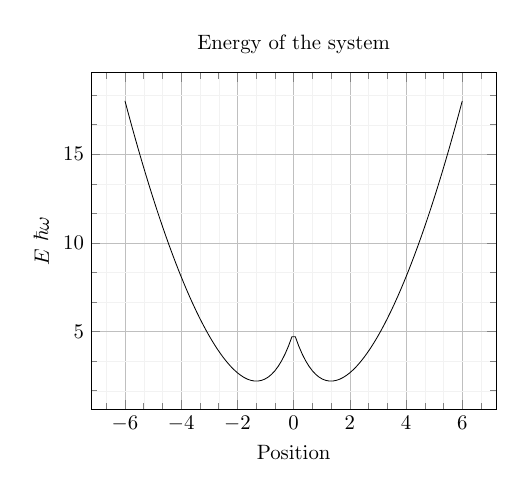
\begin{tikzpicture}[scale = 0.75]
            \begin{axis}[
                    xlabel = {Position},
                    ylabel = {$E$ $\hbar\w$},
                    title = {Energy of the system},
                    grid = both,
                    grid style={line width=.1pt, draw=gray!10},
                    major grid style={line width=.2pt,draw=gray!50},
                    minor tick num=2,
                    legend pos = north west,
                    domain = -6:6,
                    samples = 100,
                ]
                \addplot[thin, black] {x*x / 2 + 10 * exp(-abs(x)) / 2};
            %\addplot[thin, blue] {x^2/2} node[pos = 0.5, above] {$V(x)$};
            \end{axis}
        \end{tikzpicture}
        \caption{Potential of the system.}
        \label{fig: potential modified}
    \end{subfigure}
    \hfill
    \begin{subfigure}{0.45\textwidth}
        \begin{tikzpicture}[scale = 0.75]
            \begin{axis}[
                    xlabel = {Position},
                    ylabel = {$\abs{\psi}^2$},
                    title = {Probability distribution $\abs{\psi_i}^2$},
                    grid = both,
                    grid style={line width=.1pt, draw=gray!10},
                    major grid style={line width=.2pt,draw=gray!50},
                    minor tick num=2,
                    legend pos = north west,
                ]
                \addplot[thin, blue] table [x index = 0, y index = 1, header = true] {code/5pt_modified.dat};
                \addlegendentry{$\psi_0$};
                \addplot[thin, red] table [x index = 0, y index = 2, header = true] {code/5pt_modified.dat};
                \addlegendentry{$\psi_1$};
                \addplot[thin, dashed, black] table [x index = 0, y index = 3, header = true] {code/5pt_modified.dat};
                \addlegendentry{$\psi_2$};
                \addplot[thin, dashed, purple] table [x index = 0, y index = 4, header = true] {code/5pt_modified.dat};
                \addlegendentry{$\psi_3$};
            \end{axis}
        \end{tikzpicture}
        \caption{Probability distribution of the system.}
        \label{fig: potential modified probability}
    \end{subfigure}
    \caption{Potential and probability distribution of the modified potential}
    \label{fig: modified system}
\end{figure}\noindent
The eigen-values corresponding to the four first eigen-states are given in the table below.
\begin{table}[H]
    \centering
    \caption{Eigen-values of the modified potential}
    \begin{tabular}{|c|c|}\hline
        Eigen-state & Eigen-value [$\hbar\w$]\\\hline
        0 & $2.893$\\
        1 & $3.030$\\
        2 & $4.246$\\
        3 & $4.725$\\\hline
    \end{tabular}
\end{table}


\begin{figure}
    \centering
    \begin{tikzpicture}
        \begin{axis}[
                xlabel = {Position},
                ylabel = {$\psi$},
                grid = both,
                grid style={line width=.1pt, draw=gray!10},
                major grid style={line width=.2pt,draw=gray!50},
                minor tick num=2,
                title = {Wave function $\psi_i$},
                legend pos = south east,
            ]
            \addplot[thin, loosely dashed, black] table[x index = 0, y index = 1, header = true] {code/dm_wave.dat};
            \addlegendentry{$\psi_0^{d}$};
            \addplot[thin, dashed, blue] table[x index = 0, y index = 3, header = true] {code/dm_wave.dat};
            \addlegendentry{$\psi_2^{d}$};
            \addplot[thin, densely dotted, black] table [x index = 0, y index = 1] {code/ipm_wave.dat};
            \addlegendentry{$\psi_0^{i}$};
            \addplot[thin, densely dotted, blue] table [x index = 0, y index = 2] {code/ipm_wave.dat};
            \addlegendentry{$\psi_2^{i}$};
        \end{axis}
    \end{tikzpicture}
    \caption{Wave function for the iterative method $\psi_i^i$ and the direct method $\psi_i^d$.}
    \label{fig: difference between iterative and direct wavefunction}
\end{figure}



\section{Conclusion}

\section{Appendix}


\end{document}
 
